\documentclass[11pt]{article}

\newcommand{\lectureNum}{03}
\newcommand{\lectureName}{Data Formats \& Encoding II}
\newcommand{\lectureDate}{2024-01-29}

\usepackage{../dbnotes}
\usepackage{float,array}
\usepackage[table]{xcolor}
\definecolor{headerColor}{gray}{0.9}
\definecolor{headerColor2}{gray}{0.8}

\crefname{figure}{figure}{figures}


\begin{document}

\maketitle
\thispagestyle{plain}

%% ==================================================================
%% INTRODUCTION
%% ==================================================================
\section{Introduction}
Continuing with our study of analytics workloads in the cloud and data moving into data lakes that reside on object storage services like S3, we look at more storage formats based on the Partition Attributes Across (PAX) hybrid storage model. In the previous lecture, we also covered the N-ary and decomposition storage models. Rather than storing all the attributes for a single tuple contiguously in a single page (in the case of N-ary), or storing a single attribute for all tuples in a block of data (with decomposition), PAX vertically partitions attributes within a database page.

We covered open storage formats like Apache Parquet based on PAX that support this new cloud data warehousing paradigm. However, many existing formats are not optimized for remotely-accessed datalakes and today's high-throughput networks. In this lecture, we explore several modern
storage formats that make use of recent advances in networked storage and data-parallel CPU architectures.

In particular, we will look at the following storage formats:
\begin{enumerate}
    \item BtrBlocks~\cite{btrblocks} (from the Technical University of Munich)
    \item FastLanes~\cite{fastlanes} (from the Centrum Wiskunde \& Informatica in The Netherlands)
    \item BitWeaving~\cite{bitweaving} (from the University of Wisconsin)
\end{enumerate}

\section{BtrBlocks}
The BtrBlocks paper argues that inefficient decompression with formats like Apache Parquet makes scans CPU-bound and increases query time and cost. To address this, BtrBlocks uses additional encoding schemes for different data types. However, the effectiveness of these encodings differs depending on the data distribution. Given a set of encodings, we also need an algorithm for deciding which encoding is most effective for a specific data block.

\subsection{Overview}
BtrBlocks is an open columnar storage format designed for data lakes. It is designed to minimize the overall workload cost through low storage costs and fast decompression. It uses more aggressive nested encoding schemes than Parquet and ORC\@. It uses seven existing and one new encoding scheme for floating-point values.

BtrBlocks uses a greedy algorithm to select the best encoding for a column chunk, based on sampling, and then recursively tries to encode outputs of that encoding. The benchmarks in the paper show scans on real-world data are 2.2\texttimes\ faster and 1.8\texttimes\ cheaper when using BtrBlocks over Parquet. BtrBlocks stores a file's meta-data separately from the data, arguing for the ability to prune data using statistics and indices before accessing a file through a high-latency network.

\subsection{Sampling technique}

BtrBlocks collects a sample from the data and then tries out all viable encoding schemes for three rounds. Samples are collected by selecting multiple small runs from non-overlapping random positions. The BtrBlocks paper finds that sampling multiple small chunks across the entire block improves accuracy, although there is little difference between strategies that choose chunks of $\geq 16$ tuples. The intuition is that the sample needs to capture both \textbf{data locality} and \textbf{data distribution} across the entire block.

\subsection{Encoding schemes}

BtrBlocks selected the following encoding schemes by analyzing a collection of real-world datasets:

\begin{itemize}
    \item \textbf{Run-length encoding (RLE) \& One Value}: involves storing the run $(42,3)$ instead of $\{42, 42, 42\}$. One value is an extreme case for columns with only one unique value per block.
    \item \textbf{Frequency encoding~\cite{freq-encoding}}: addresses skewed distributions, using several code lengths based on data frequency. For example, the two most frequent values can be represented by a one-bit code, and the next eight most frequent values using a three-bit code. BtrBlocks adapts this by only storing the top value, a bitmap encoding which values are the top value, and the exception values which are not the top value.
    \item \textbf{Frame of Reference (FOR) + Bit-packing}: FOR encodes each integer as a delta to a chosen base value, for example storing the base $100$ and $\{5,1,13\}$ instead of $\{105,101,113\}$. Useful in combination with bit-packing, which truncates unnecessary leading bits. For example, $\{5,1,13\}$ can be bit-packed using 4 bits for each value instead of 8.
    \item \textbf{Dictionary encoding}: covered in the previous lecture
    \item \textbf{Fast static symbol table (FSST)}: see \cref{sec:fsst}
    \item \textbf{Roaring bitmaps for NULLs + exceptions}: see \cref{sec:roaring}
    \item \textbf{Pseudodecimals}: see \cref{sec:pseudo}
\end{itemize}

Note that these encoding schemes can be used in a cascade. For example, you could encode with RLE and then with bit-packing.

\subsubsection{Fast static symbol table (FSST)}\label{sec:fsst}
In many real-world databases strings form a large fraction of data. Strings are often compressed using dictionaries. However, since dictionary compression uniquely maps strings to fixed-size integers, compression can be sub-optimal on data that has many unique values that might be similar but not equal. Further, DBMSs benefit from random access to individual string attributes, which is not possible when using block-wise general string compression like LZ4. FSST, introduced by Boncz et al.~\cite{fsst}, is a string encoding scheme that supports random access without decompressing previous entries. It replaces frequently occurring substring (up to 8 bytes) with 1-byte codes. It uses a ``perfect'' hash table for fast look-up of symbols without conditionals and loops.

\begin{figure}[H]
    \centering
    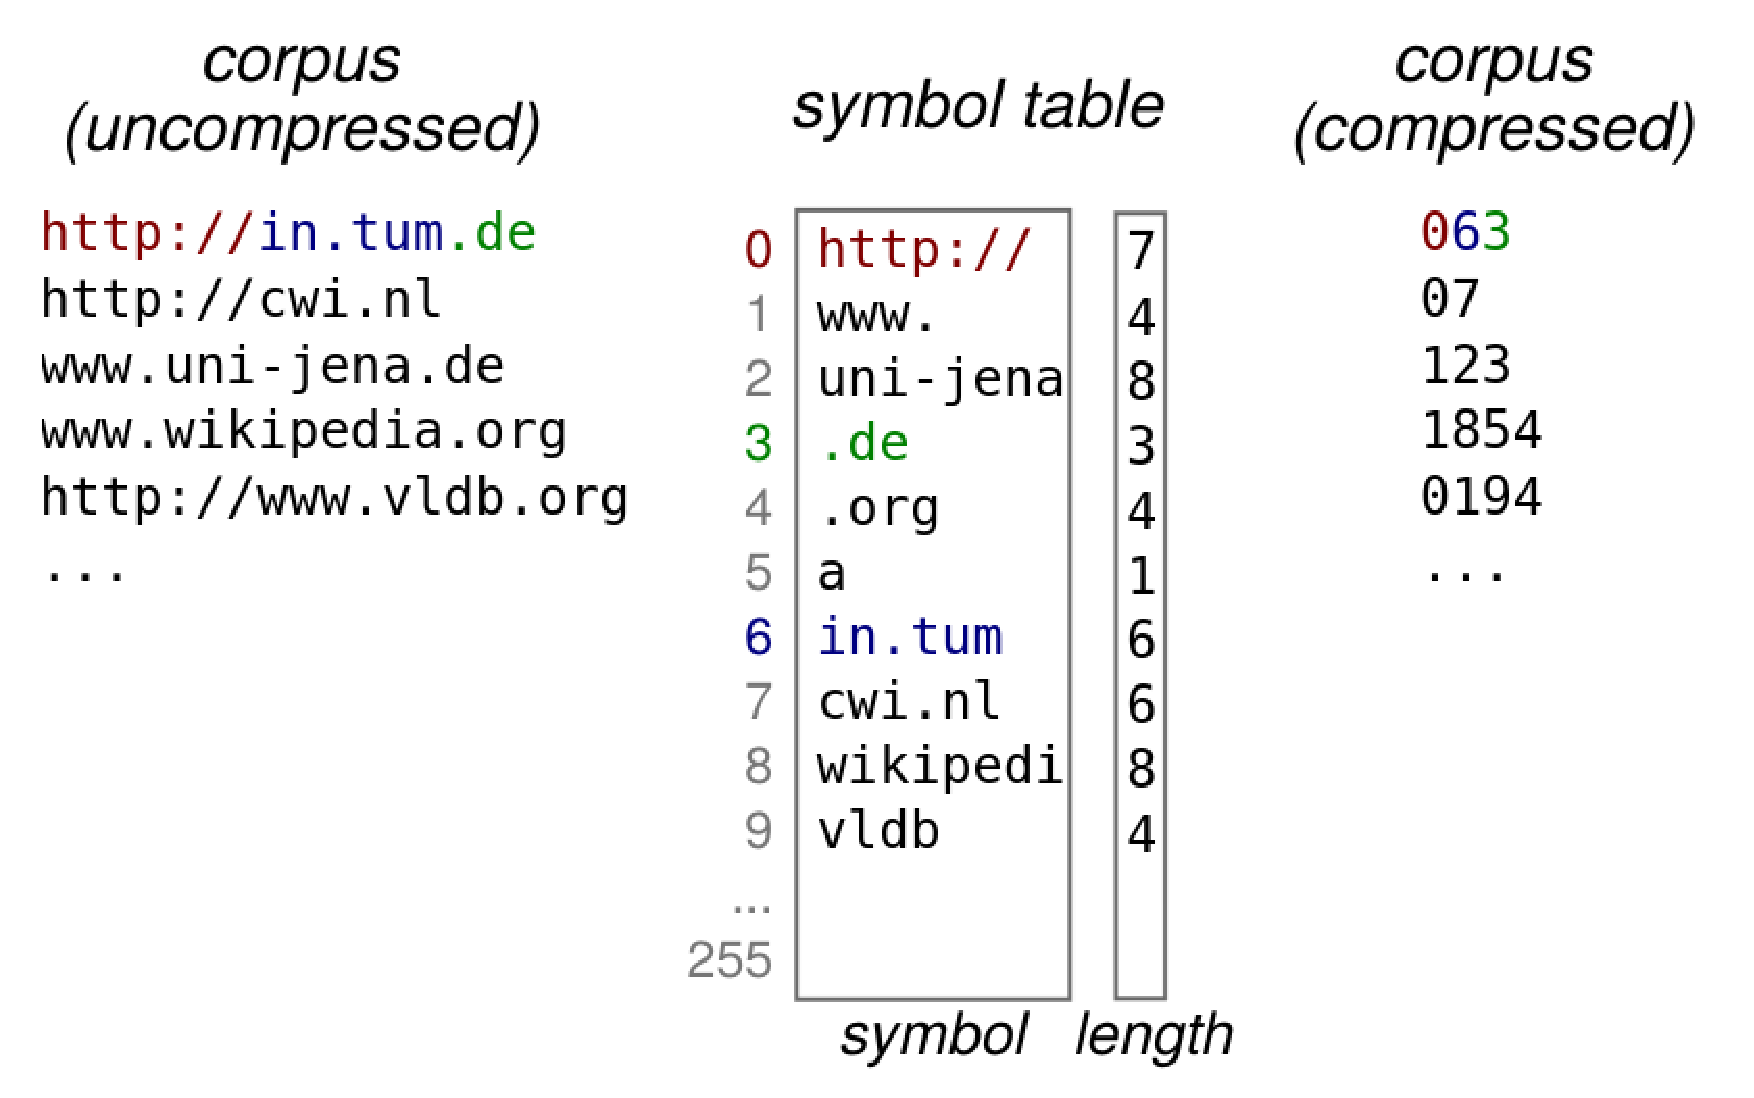
\includegraphics[width=0.5\linewidth]{fig/fsst-example.pdf}
    \caption{Symbols of length 1-8 are replaced with 1-byte codes. Performance is dependent on finding a good symbol table.}\label{fig:fsst-example}
\end{figure}

FSST constructs a symbol table using an evolutionary algorithm. Consider an example for encoding the string ``tumcwitumvldb''.
\begin{figure}[H]
    \centering
    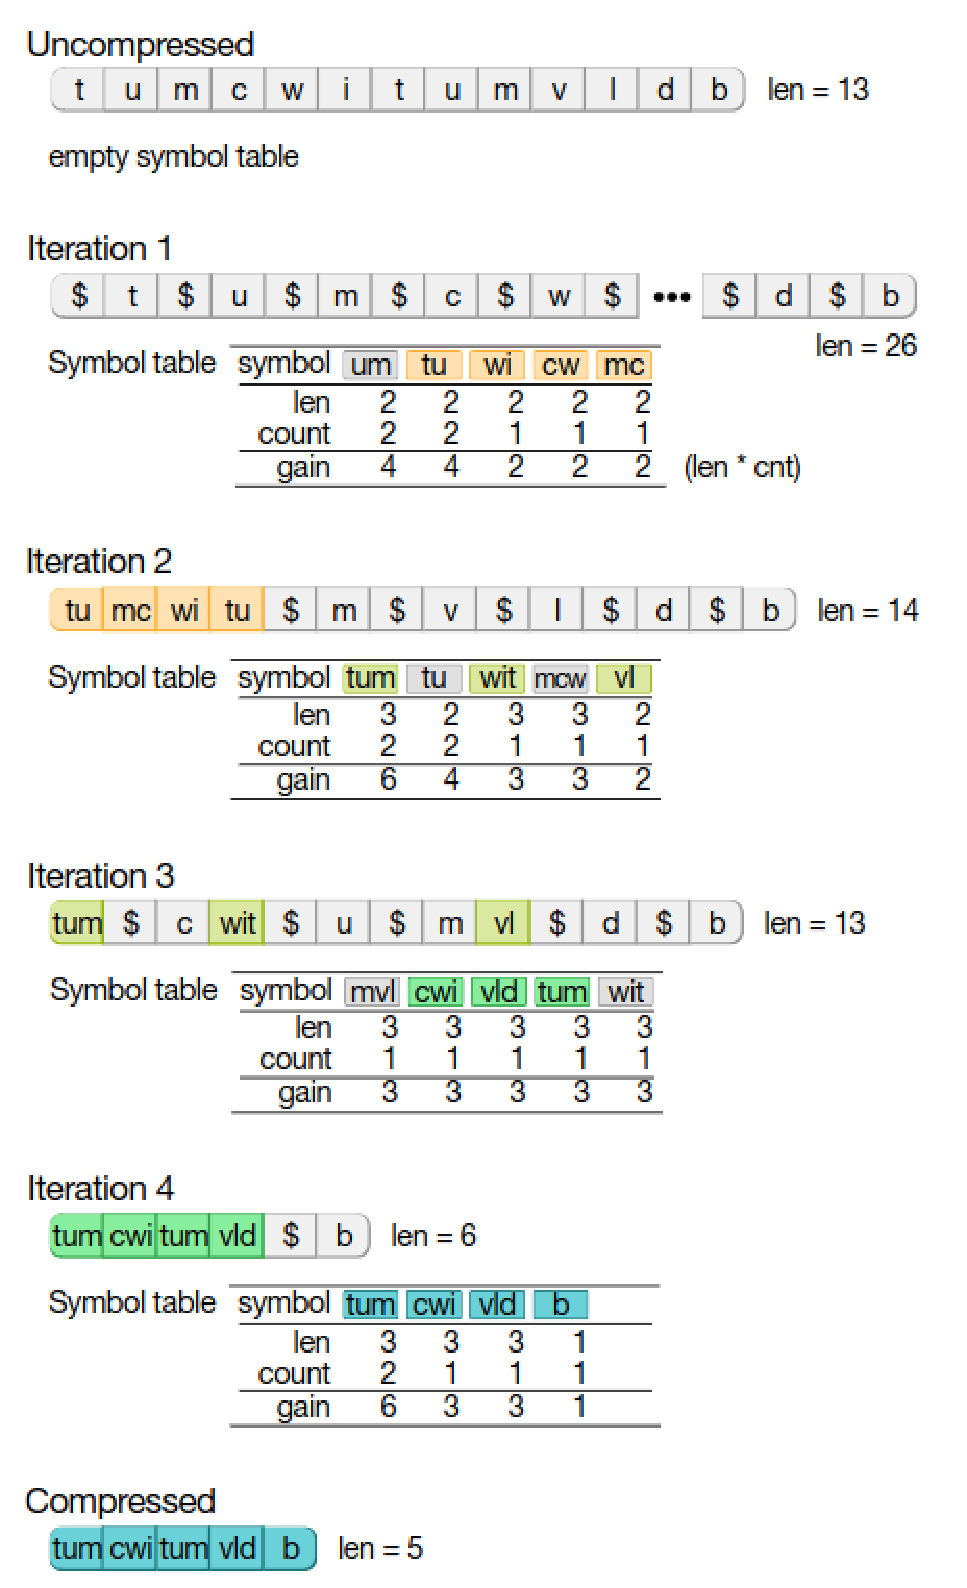
\includegraphics[width=0.4\linewidth]{fig/fsst-algo.pdf}
    \caption{FSST symbol table construction algorithm}\label{fig:fsst-algo}
\end{figure}
Assume we only look at symbols that are at most 3 characters long, and that the symbol table can have at most 5 entries. The algorithm proceeds in multiple iterations, starting with an empty symbol table as shown in \cref{fig:fsst-algo}. In each iteration the compressed string is shown at the top, compressed using the previous iteration's symbol table, with '\$' used to depict the escape byte needed to escape each symbol. In the beginning, with an empty symbol table, the length of the compressed string doubles because we must escape each symbol. Each new iteration does two things. First, it computes the compression factor using the current symbol table. This step also counts how often each symbol occurs in the compressed string and the symbols that appear in succession. Second, a new symbol table is constructed by selecting the symbols with the highest apparent gains (number of occurrences * symbol length), including new symbols generated by concatenating pairs of successive symbols found in the compressed string. The idea is that frequently occurring longer, higher-gain symbols found in this manner will replace less worthwhile symbols from the previous iteration.

For example, in iteration 2, we generate the symbol \texttt{tum}, from successively occurring symbols \texttt{tu} and \texttt{mc}, which has higher gains than any other symbols from the symbol table from iteration 1.\ \texttt{tum} ends up replacing the symbol \texttt{um}, with ties broken arbitrarily.

\subsubsection{Roaring bitmaps for NULLs + exceptions}\label{sec:roaring}
Roaring bitmaps, introduced by Chambi et al.~\cite{Chambi_2015}, are bitmap indices that switch which data structure to use for a range of values depending on the local density of bits. Dense chunks are stored using uncompressed bitmaps. Sparse chunks are stored using bit-packed arrays of 16-bit integers.

Roaring partitions the space $[0,n)$ into chunks of $2^{16}$ integers ($[0,2^{16}),[2^{16},2\times 2^{16}),\ldots$). Dense chunks, containing more than $4096$ integers, are stored using conventional bitmap containers (made of $2^{16}$ bits or $8$kB) whereas sparse chunks use smaller containers made of packed sorted arrays of 16-bit integers.

\begin{figure}[H]
    \centering
    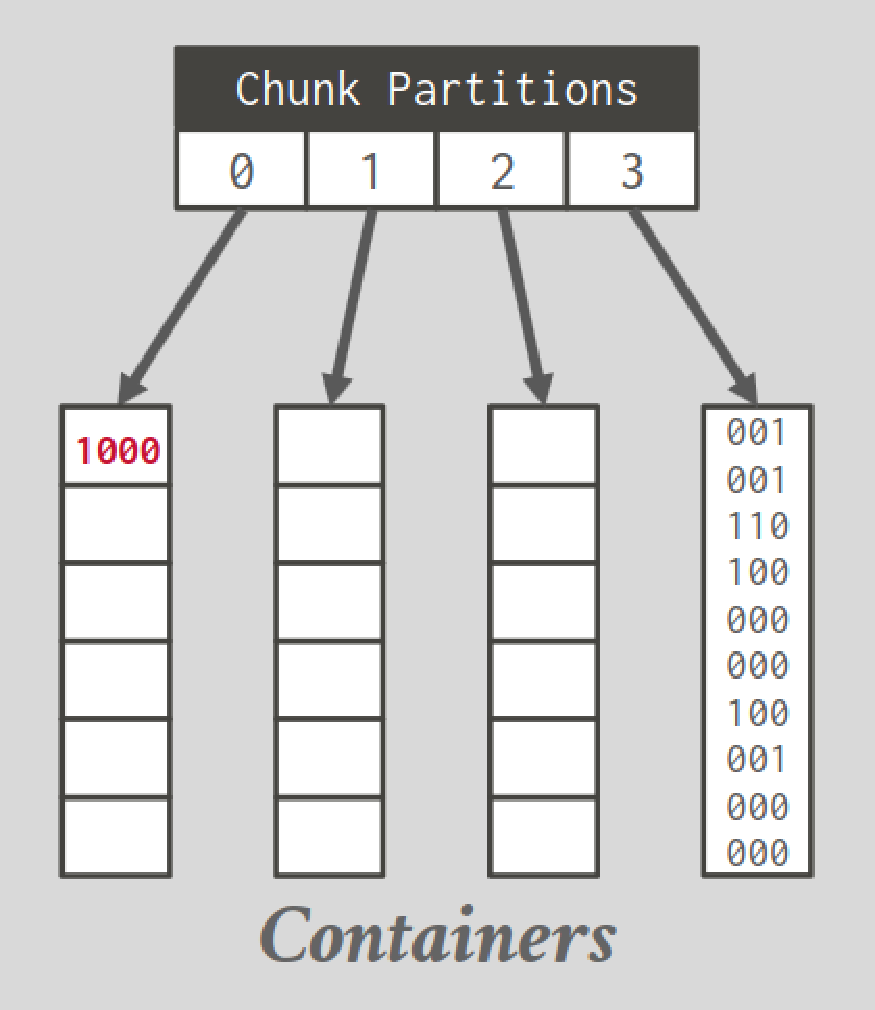
\includegraphics[width=0.3\linewidth]{fig/roaring.pdf}
    \caption{Roaring bitmap example}\label{fig:roaring-example}
\end{figure}

In \cref{fig:roaring-example}, to insert the value $1000$, we first find the chunk associated with it. Since $\lfloor1000/2^{16}\rfloor=0$, it will be inserted in the first container. Since there are no values in the first chunk yet we will store this value in an array container. If we wanted to insert the value $199658$, we would follow the same process, computing $\lfloor{199658/2^{16}}\rfloor = 3$. This time, let's say there are at least $4096$ values in the third container so we are using a bitmap. Then we will simply go ahead and just set the $199658\bmod 2^{16}=3050$th bit.

BtrBlocks uses roaring bitmaps for storing \texttt{NULL} values for each column as well as for exceptions in frequency encoding.

\subsubsection{Pseudodecimals}\label{sec:pseudo}
There has not been a lot of interest in floating-point compression until now because relational systems typically represent real numbers as \texttt{Decimal} or \texttt{Numeric}, which can be physically stored as integers. However, this is changing with the move to data lakes and the subsequent integration with non-relational systems. For example, Tableau's internal analytical DBMS encodes all real numbers as floating-point numbers and machine-learning systems rely on floating-point numbers.

Pseudodecimal encoding uses a decimal representation for encoding doubles, using two integers: \textit{significant digit with sign} and \textit{exponent}. For example, $3.25$ becomes $(+325, 2)$. And for $0.99$ the encoding stores $(+99,2)$. The encoding algorithm determines the compact decimal representation by testing all powers of $10$ and checking whether any of them correctly multiply the double to an integer value. The algorithm creates exceptions for values like negative zero, $\pm\infty$, and $\pm NaN$, as well as extremely small values like $5.5\times 10^{-42}$ that it cannot successfully encode. Refer to the BtrBlocks paper for details about the encoding and decoding process.

Pseudodecimal encoding is not well-suited for columns with many exception values, or columns with few unique values. Columns with few unique values compress almost as well by using dictionary encoding.
\section{FastLanes}
BtrBlocks, Parquet, and ORC generate variable-length runs of values. This wastes cycles during decoding for both scalar and vectorized operations. Parquet and ORC, in particular, use Delta encoding where each tuple's value depends on the preceding tuple's value. This is impractical to process with SIMD because you cannot pass data between lanes in the same register.

FastLanes is a suite of encoding schemes that achieve better data parallelism through clever reordering of tuples to maximize useful work in SIMD operations. These algorithms can be emulated on AVX512 or scalar instructions. The FastLanes authors define a ``virtual'' ISA with 1024-bit SIMD registers, designed to operate on any current and future register widths. FastLanes' novel ``Unified Transposed Layout'' exploits the property of relational algebra that it is based on unordered sets.

\subsection{Background: Sequential Data Dependencies}
Delta encoding, particularly when combined with run-length encoding, can yield immense compression ratios for some data types. However, the canonical Delta model is largely sequential because it relies on computing the accumulated differences between neighboring values in the data layout.

\begin{figure}[H]
    \centering
    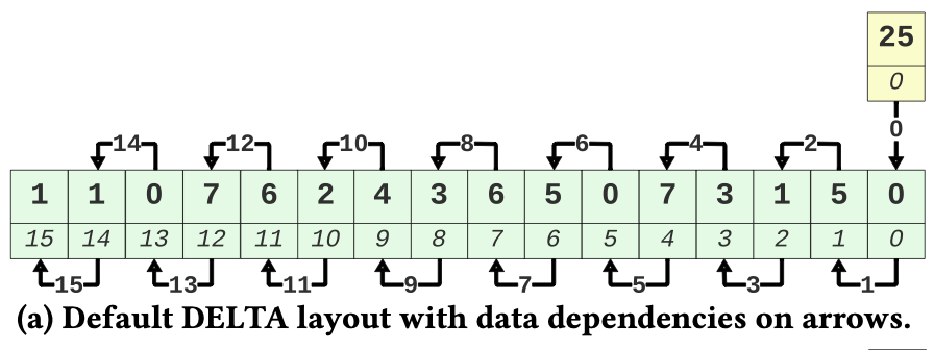
\includegraphics[width=0.5\linewidth]{fig/default-delta.pdf}
    \caption{Sequential data dependencies in the default Delta layout.}\label{fig:default-delta}
\end{figure}

\Cref{fig:default-delta} illustrates the data dependencies that are created across multiple vector lanes. Even with a large register capable of holding many values, the CPU cannot make maximal use of SIMD parallelism because it still must iteratively calculate the deltas across its lanes.

\subsection{The Unified Transport Layout}
Upon decoding, FastLanes makes a critical adjustment to the data layout. First, it splits the data into many sequential runs, which in practice consists of 16 sets of 8 sequential values. Each run begins with its own \textit{base} value (shown in yellow), which differs from the default format, which only has one base value.

It then reorders the values, moving each base value to the front, and then shifting over chunks of sequential values starting from each base value.\ \cite{fastlanes}

\begin{figure}[H]
    \centering
    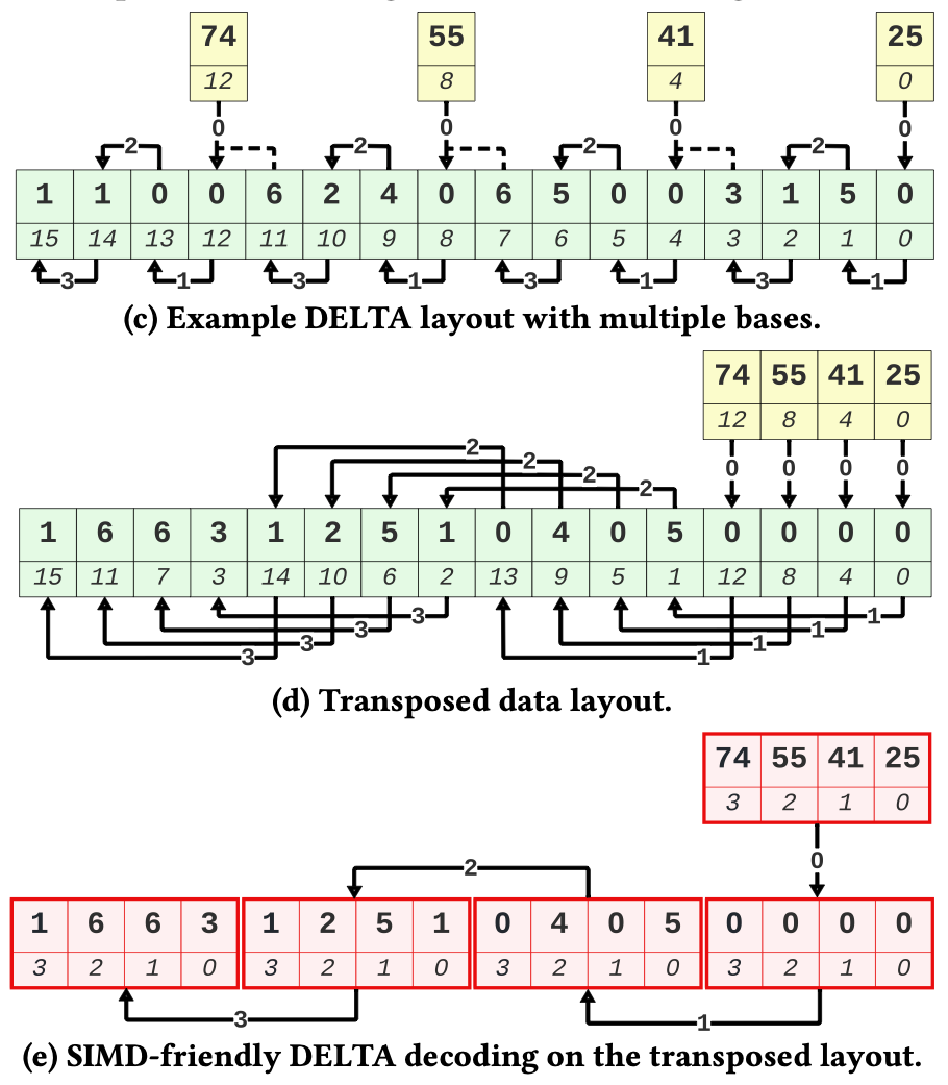
\includegraphics[width=0.5\linewidth]{fig/reordered-delta.pdf}
    \caption{Improved Delta format with UTL.}\label{fig:reordered-delta}
\end{figure}

\Cref{fig:reordered-delta} shows an example of the reordering. Values 0, 4, 8, and 12 are designated as the base values and are reordered to the front of the layout in step (d). Each of their dependencies, values 1, 5, 9, and 13, are moved to the next chunk over, and so on. With this transposing of data, resolving the Delta values only takes three SIMD additions on a vector that holds four values, rather than 15 additions.

\subsection{A Portable SIMD Interface}
There are two main challenges with designing SIMD-targeted software:
\begin{itemize}
    \item \textbf{Varying SIMD Widths:} Modern ISAs have different register widths, ranging from 64 bits to 512 bits and possibly more. Furthermore, the FastLanes authors note that SIMD ISAs have widened dramatically in the past 25 years (by a factor of 8), and this trend is likely to continue in the future.
    \item \textbf{Heterogeneous ISAs:} SIMD instructions are specific to each architecture. Although high-level code can often emit SIMD instructions via compiler intrinsics, this approach is not portable across architectures. Additionally, the set of logical SIMD instructions may not be supported in some architectures; therefore, some approaches that rely on specific bitwise operators may not work on unsupported ISAs.
\end{itemize}
FastLanes resolves these challenges by introducing a ``virtual instruction set'' called \texttt{FLMM1024} which simulates operations on a 1024-bit register set. This virtual ISA is comprised of a minimal set of 1024-bit operations (\texttt{LOAD, STORE, AND, XOR, ADD}, etc.) that can fully execute data-parallel FastLanes decoding.

\begin{figure}[H]
    \centering
    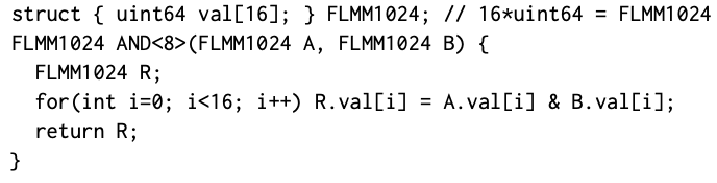
\includegraphics[width=0.6\linewidth]{fig/flmm-code.pdf}
    \caption{An example of the FLLM1024 AND instruction.}\label{fig:flmm-code}
\end{figure}

FLMM instructions consist of a simple loop that executes basic C bitwise operators. This approach relies on the fact that modern optimizing compilers can auto-vectorize suitable code, ensuring that any architecture will be able to run FastLanes on the widest registers available.

\section{BitWeaving}
The encoding schemes we have discussed so far scan data by examining the entire value of each attribute and cannot short-circuit comparison with integer types, known as \textit{early pruning}, because CPU instructions operate on entire words. Further, modern CPUs have a word width of 64 bits but values in a database table column are often represented with fewer bits. This leads to underutilization of the width of a word. In the case of SIMD, compressed column values are often packed into four 32-bit slots in a 128-bit SIMD word~\cite{simdfastscan}. But for compressed values encoded with fewer bits, this still requires padding the values to 32-bit boundaries. This means that even with state-of-the-art techniques it still takes many cycles per input tuple to apply simple predicates on a single column of a table.

\subsection{Background: Bit-sliced encoding}
Noting the read-mostly environment of data warehousing, O'Neil et al.~\cite{varindexes} introduced a bit-sliced indexing method taking an orthogonal bit-by-bit view of the same data. Consider the following data:

\begin{table}[!htbp]
\rowcolors{2}{headerColor}{white}
\begin{tabular}{|c|c|}
\hline
\rowcolor{headerColor2}
id & zipcode \\
\hline
1 & 21042 \\
2 & 15217 \\
3 & 02903 \\
4 & 90220 \\
5 & 14623 \\
6 & 53703 \\
\hline
\end{tabular}
\end{table}
And the following query:
\begin{lstlisting}[language=SQL]
SELECT * FROM customer_dim
WHERE zipcode < 15217
\end{lstlisting}

Instead of having to query all the bits of each zip code with 15217, we could represent the zip codes as \textit{bit slices}:

\begin{table}[!htbp]
\rowcolors{2}{headerColor}{white}
\begin{tabular} {|c|c|c|c|c|c|c|c|c|c|c|c|c|c|c|c|c|c|}
\hline
\rowcolor{headerColor2}
null & 16 & 15 & 14 & 13 & 12 & 11 & 10 & 9 & 8 & 7 & 6 & 5 & 4 & 3 & 2 & 1 & 0 \\
\hline
0 & 0 & 0 & 1 & 0 & 1 & 0 & 0 & 1 & 0 & 0 & 0 & 1 & 1 & 0 & 0 & 1 & 0 \\
\hline
0 & 0 & 0 & 0 & 1 & 1 & 1 & 0 & 1 & 1 & 0 & 1 & 1 & 1 & 0 & 0 & 0 & 1 \\
\hline
0 & 0 & 0 & 0 & 0 & 0 & 1 & 0 & 1 & 1 & 0 & 1 & 0 & 1 & 0 & 1 & 1 & 1 \\
\hline
0 & 1 & 0 & 1 & 1 & 0 & 0 & 0 & 0 & 0 & 0 & 1 & 1 & 0 & 1 & 1 & 0 & 0 \\
\hline
0 & 0 & 0 & 0 & 1 & 1 & 1 & 0 & 0 & 1 & 0 & 0 & 0 & 1 & 1 & 1 & 1 & 1 \\
\hline
0 & 0 & 1 & 1 & 0 & 1 & 0 & 0 & 0 & 1 & 1 & 1 & 0 & 0 & 0 & 1 & 1 & 1 \\
\hline
\end{tabular}
\end{table}
Each bit slice can be represented as a bitmap, and the bit-sliced index for the \texttt{zipcode} column is just the set of these bitmaps. To execute the range query with this bit-sliced representation, we can walk each slice and construct a result bitmap that skips entries that have a 1-bit set in the first three slices (16, 15, and 14) since 15217 only has 14 bits in its binary representation.

These bit slices can also be used for efficient aggregate computations, for example, to calculate the sum of a column using hamming weight. This algorithm would process as follows:
\begin{enumerate}
    \item Count the number of 1-bits in the slice in base-17, and multiply the count by $2^{17}$
    \item Count the number of 1-bits in the slice in base-16, and multiply the count by $2^{16}$
    \item And so on for the remaining slices..
\end{enumerate}
The \texttt{POPCNT} instruction can be used to efficiently count the number of 1-bits in a register.

BitWeaving improves upon the bit-sliced index with a new storage layout that is optimized for memory access and early pruning.

\subsection{Overview}
BitWeaving is an encoding scheme for columnar databases that supports efficient predicate evaluation on compressed data using SIMD\@. It was implemented in the Quickstep~\cite{quickstep} engine. It aims to aggressively exploit \textit{intra-cycle} parallelism in main-memory analytic DBMSs. The idea is that even within a single processor cycle there is abundant parallelism as the circuits in the processor core are simultaneously computing on multiple bits of information, even when working on simple ALU operations. The technique tries to exploit this parallelism to process data at or near the speed of the processor.


\subsection{Mechanism}
BitWeaving exploits the parallelism available at the bit level in modern processors. It does not rely on hardware-implemented SIMD capability. There are two flavors of BitWeaving:
\begin{figure}[H]
    \centering
    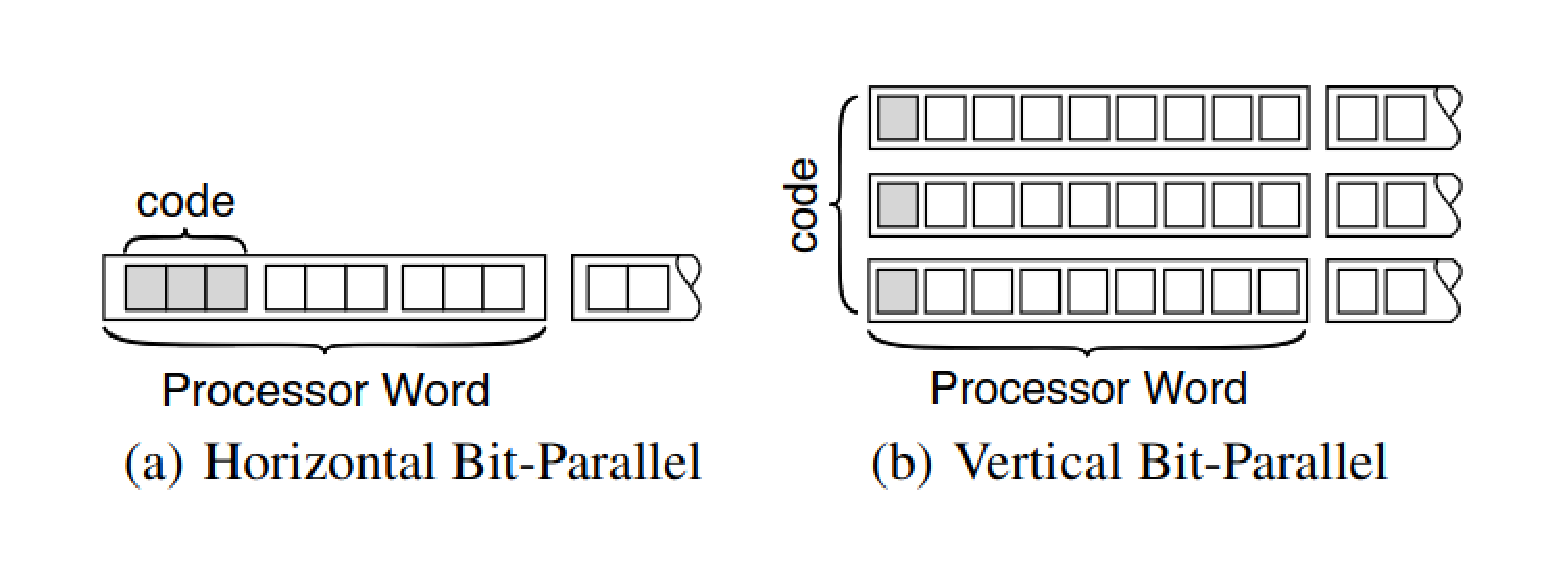
\includegraphics[width=0.5\linewidth]{fig/bitweaving-flavors.pdf}
    \caption{BitWeaving/H and BitWeaving/V layouts for column values encoded with 3 bits.}\label{fig:bitweaving-flavors}
\end{figure}
\begin{itemize}
    \item \textbf{BitWeaving/V}: uses bit-level columnar data organization, packed into processor words. However, looking up a value can incur many CPU cache misses and hurt performance as all the bits of a value are spread out.
    \item \textbf{BitWeaving/H}: all the bits of a column value are stored together. This provides high performance when fetching the entire column value but uses an additional bit as a delimiter between adjacent values. In extreme cases, this flavor can be 2\texttimes\ slower than BitWeaving/V because of this additional bit that prevents it from storing two 32-bit values in a 64-bit processor word. Further, this flavor does not perform early pruning as that would require performing extra processing that impacts performance.
\end{itemize}

\subsection{Filtering with BitWeaving: Examples}
The following illustrates an example of how columnar scans with predicates can be accelerated using BitWeaving on 3-bit tuples with an 8-bit word size. The advantage of this approach is that it requires minimal instructions to evaluate a predicate on many tuples at once.

We will consider the following query on a table with 10 tuples:
\begin{lstlisting}[language=SQL]
SELECT * FROM TABLE
WHERE val < 5
\end{lstlisting}

\begin{itemize}
    \item \textbf{BitWeaving/H:}
    \begin{figure}[H]
    \centering
    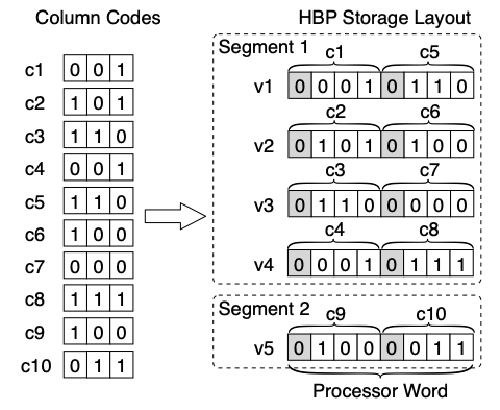
\includegraphics[width=0.5\linewidth]{fig/horiz-layout.pdf}
    \caption{The BitWeaving horizontal storage layout.}\label{fig:horiz-layout}
    \end{figure}
    The first step in the horizontal model is to pack the column values into registers with a 1-bit delimiter, initially zero, prefixed to each value. Ordering the 1st and 5th values together, then the 2nd and 6th, etc.\ will enable us to produce a selection vector very efficiently after the predicate is evaluated.
    \begin{figure}[H]
    \centering
    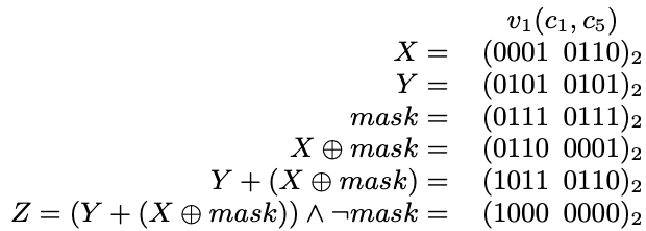
\includegraphics[width=0.5\linewidth]{fig/horiz-procedure.pdf}
    \caption{Evaluating the predicate $c < 5$.}\label{fig:horiz-procedure}
    \end{figure}
    Now we evaluate the predicate. This is done by creating a constant word $Y$ containing two instances of the filter comparison constant 5 from the query, as well as a $mask$ with ones everywhere but the delimiter. We then take $Y + (X \oplus mask)$, which has the effect of computing $5 + (2^3 - X - 1)$ since both $X\oplus mask$ and $2^3-X-1$ compute the 3-bit logical complement of $X$. This sets the delimiter only if $X \leq 5-1=4$. Filtering the result with the complement of $mask$ leaves us with just the delimiters.

    \begin{figure}[H]
    \centering
    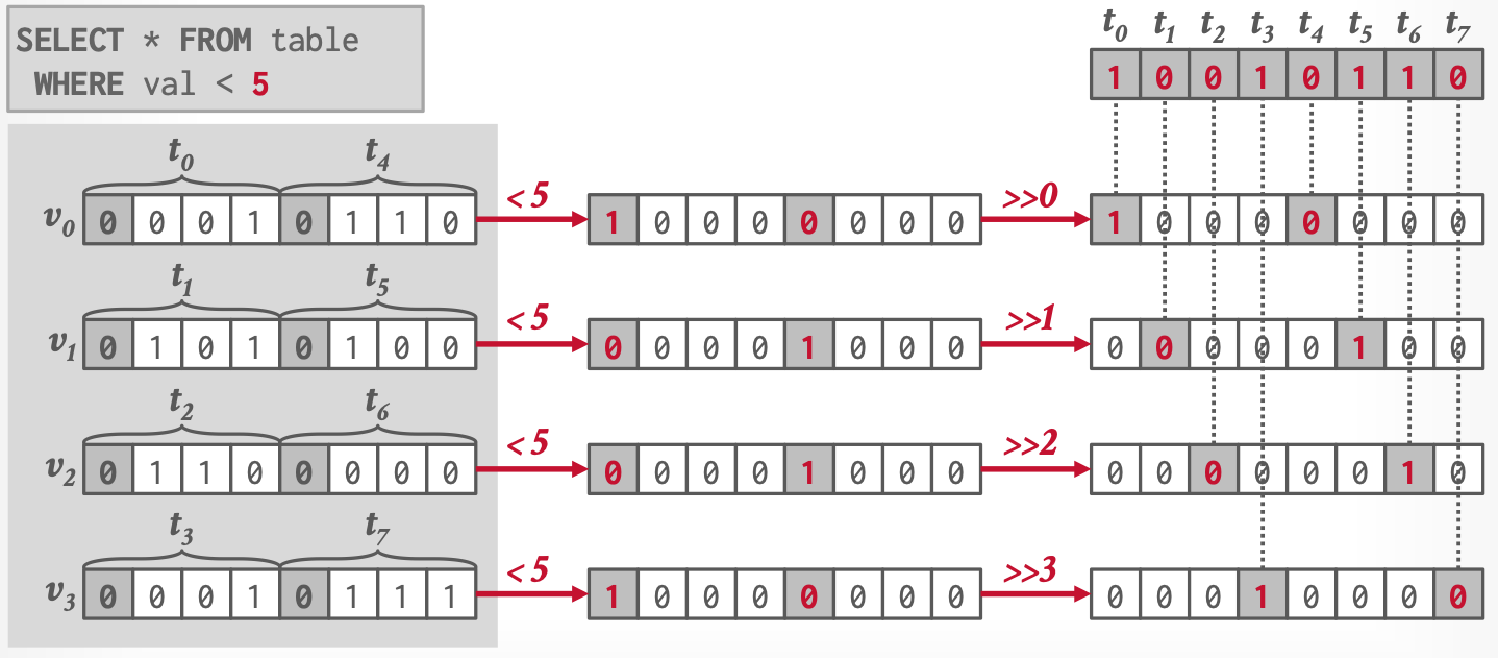
\includegraphics[width=0.8\linewidth]{fig/selection-vector.pdf}
    \caption{Generating the selection vector.}\label{fig:selection-vector}
    \end{figure}
    The horizontal layout requires an additional step to generate the selection vector. The original tuples were reordered in the horizontal layout such that this can be accomplished in a short series of shifting operations.

    \item \textbf{BitWeaving/V:}
    \begin{figure}[H]
    \centering
    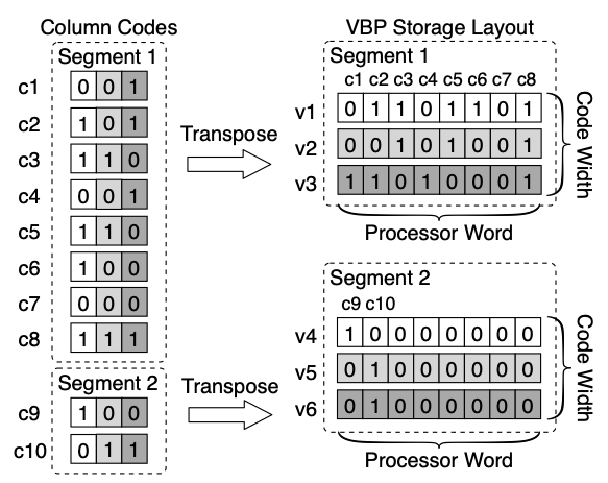
\includegraphics[width=0.5\linewidth]{fig/vert-transpose.pdf}
    \caption{The BitWeaving vertical storage layout.}\label{fig:vert-transpose}
    \end{figure}
    The vertical model instead transposes sequential column values into a series of words divided by bit order, so the most significant bits of each value are stored in the same word. This method is not sensitive to the size of column values and does not require a delimiter.

    \begin{figure}[H]
    \centering
    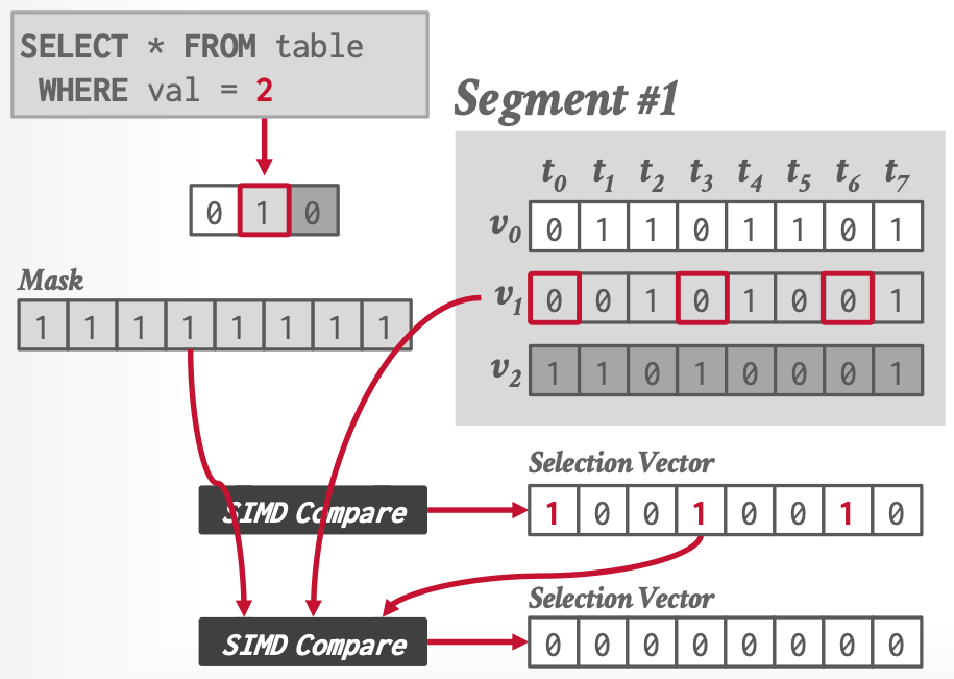
\includegraphics[width=0.5\linewidth]{fig/vert-compare.pdf}
    \caption{Evaluating the predicate $v = 2$.}\label{fig:vert-compare}
    \end{figure}
    As with the horizontal layout, we construct constant-value masks to compare multiple tuples in parallel. The algorithm considers one bit position of the lookup value at a time. This time, each mask consists entirely of the bit at the position being evaluated: to compare against the value 2, we compare all most significant bits to the value 0, using \texttt{xor} and \texttt{and} operations to update the selection vector. This process is repeated for all bit positions until the end is reached or, critically, as soon as the selection vector equals zero.

\end{itemize}

Both BitWeaving/V and BitWeaving/H produce as output a result bit vector, with one bit per input tuple that indicates if the tuple matches the predicate on the column. This result bit vector must be converted to column offsets, which can either be done using iteration or a pre-computed positions table (see \cref{fig:bitweaving-positions-table}). BitWeaving/V outperforms BitWeaving/H for scan performance whereas BitWeaving/H achieves better lookup performance.

\begin{figure}[H]
    \centering
    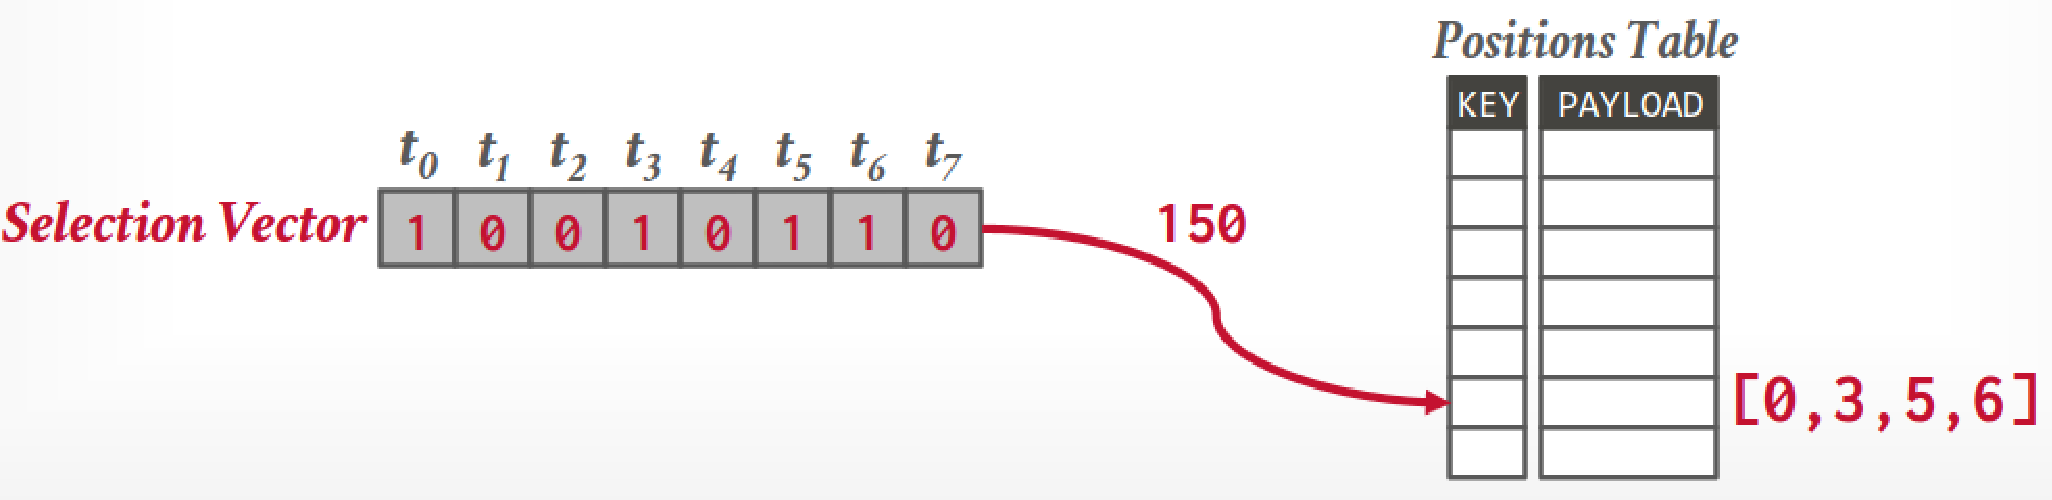
\includegraphics[width=0.75\linewidth]{fig/bitweaving-positions-table.pdf}
    \caption{Pre-computed positions table}\label{fig:bitweaving-positions-table}
\end{figure}

The key takeaway is that predicates can often be computed by only looking at some of the most significant bits in each column. The compact result bit vectors produced can also be used to evaluate the next stage of a complex predicate efficiently.

BitWeaving specifies bit-parallel algorithms that only require full-word operations common in all modern CPU architectures: logical and, logical or, exclusive or, binary addition, negation, and $k$-bit left or right shift. These methods can be used either as the primary storage organization technique in a column store database or as an indexing method to index columns.

The paper shows that BitWeaving methods outperform methods like SIMD-scanning and naive methods over all column widths, but they achieve higher speedups when the column representation has fewer bits. This is because this allows more column predicates to be computed in parallel. With each column encoded using 4 bits BitWeaving is 20\texttimes\ faster than SIMD scanning. For columns wider than 12 bits, it is 4\texttimes\ faster.

\section{Conclusion}
Logical-physical data independence is one of the key aspects of the relational model. The last two lectures have covered many strategies for representing data, each with unique compute-vs-storage tradeoffs. This data independence allows applications to remain oblivious to the underlying data representation. Fixed-size data, efficient compression, and modern SIMD hardware are critical for enabling large OLAP database systems to execute highly data-parallel queries. Internal storage optimizations such as BtrBlocks, FastLanes, and BitWeaving demonstrate how DBMSs can employ seemingly bizarre physical representations of data on a variety of modern hardware to accelerate queries even at the lowest levels of computation.
% ==================================================================
% BIBLIOGRAPHY
% ==================================================================
\newpage
\bibliographystyle{abbrvnat}
\bibliography{03-data2}

\end{document}
